\chapter{Parameter Inference}

\section{Motivation}

Building mathematical models of real world phenomenon allows for us to
simulate changes in the world without having to undertake large scale
experiments. However, once we have a model that sufficiently approximates
\emph{P. vivax} transmission
or anything else we are trying to model,
we then need to estimate what the `true' underlying parameters are.
To do this we calibrate the model against real world data such as case counts,
and prevalence surveys. Under frequentist assumptions, there is a `true' set of
parameters that if used in our model, simulated the observed data. Under a Bayesian
assumption, the parameters are considered to be random, and
This chapter explores statistical inference techniques to recover the
parameters, under both the frequentist and Bayesian frameworks.

\section{Frequentist Parameter Estimation}

Assume the model is parametrised by a set of parameters
$\btheta \in \mathbf{\Theta}$ which
we are trying to estimate by considering some observed data
$\by^\obs = (y_1^\obs, \dots, y_n^\obs).$
Consider $\by(\btheta) = (y_1(\btheta), \dots, y_n(\btheta))$
some model simulation of
$\by^\obs.$ Often the observed data has some underlying index set
$x_1, \dots, x_n,$ where $x_i$ might be something like time. In this case
we can also consider the observed data to be
$\{(x_1, y_1^\obs), \dots, (x_n, y_n^\obs)\},$ and the
model simulated data to be
$\{(x_1, y_1(\btheta)), \dots, (x_n, y_n(\btheta))\}.$

\subsection*{Least Squares Estimator}

It is common that models are not random, but instead model the mean behaviour
of a system. In this case, $\by(\btheta)$ is not random. Therefore
we can assume that $y^\obs_i = y_i(\btheta) + \varepsilon_i,$
where $\varepsilon_i$ is a random variable with some (possibly unknown)
distribution, and zero mean.

When the distribution of $\varepsilon_i$ is unknown, a common approach for
estimating $\btheta^{\LS}$ is to take the least squares estimate.

\begin{definition}[Least Squares Estimate]
    The \emph{least squares estimate} $\btheta^{\LS}$ for
    $\btheta$ is
    $$
        \btheta^{\LS}
        := \argmin_{\btheta\in\mathbf{\Theta}}
        \sum_{i = 1}^n (y_i(\btheta)- y_i^\obs)^2.
    $$
\end{definition}

\begin{example}\label{ex:LSE}
    Consider the observed data
    $\{(x_1, y_1^\obs), (x_2, y_2^\obs), (x_3, y_3^\obs)\}
        = \{(1, 2), (2, 4), (3, 4)\},$
    which we assume were generated from the model
    $y_i(\btheta) + \varepsilon_i,$ where
    $y_i(\btheta) = \theta_0 + \theta_1x_i,$ and
    $\E(\varepsilon_i) = 0.$ We derive the least squares estimate of our
    parameters $\btheta = (\theta_0, \theta_1)$ by

    \begin{align*}
        \btheta^{\LS}
        = & \, \argmin_{\btheta}
        [\sum_{i = 1}^3 (y_i(\btheta) - y_i^\obs)^2]           \\
        = & \, \argmin_{\btheta}
        [\sum_{i = 1}^3 (\theta_0 + \theta_1x_i - y_i^\obs)^2] \\
        = & \, \argmin_{\btheta}
        [(\theta_0 + \theta_1 - 2)^2 + (\theta_0 + 2\theta_1 - 4)^2
            + (\theta_0 + 3\theta_1 - 4)^2]
    \end{align*}

    Since the expanded quadratic will have positive coefficients out the front
    of $\theta_0$ and $\theta_1,$ we can solve for $\btheta^{\LS}$
    by

    \begin{align*}
        \mathbf{0}
        = & \, \frac{\partial}{\partial \btheta}
        [
            (\theta^\LS_0 + \theta^\LS_1 - 2)^2
            + (\theta^\LS_0 + 2\theta^\LS_1 - 4)^2
            + (\theta^\LS_0 + 3\theta^\LS_1 - 4)^2
        ]                                        \\
        = & \begin{bmatrix}
                6\theta^\LS_0 + 12\theta^\LS_1 - 20 \\
                12\theta^\LS_0 + 28\theta^\LS_1 - 44
            \end{bmatrix}
    \end{align*}
    And solving these two equations results in $\theta^\LS_0 = 4/3$ and
    $\theta^\LS_1 = 1.$ This can be visually seen in Figure \ref{fig:LSE}
\end{example}


\begin{figure}[htbp]
    \centering
    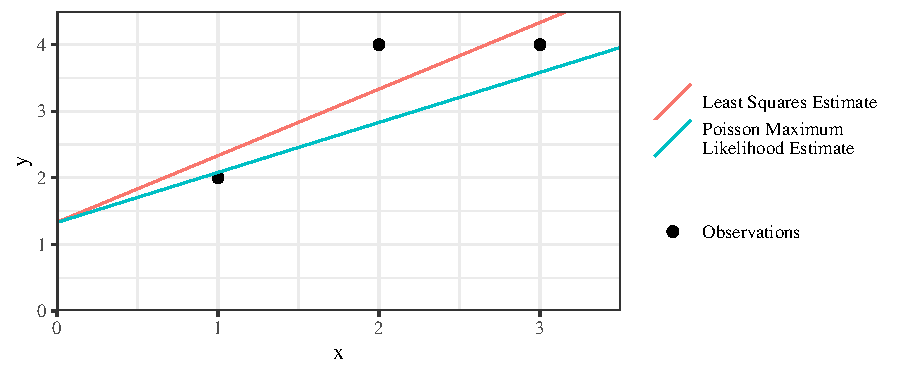
\includegraphics[width=\textwidth]{LS_example.pdf}
    \caption{
        Two linear models of the form
        $y_i(\btheta) = \theta_0 + \theta_1x_i$ fit given the set
        of observations $\{(1, 2), (2, 4), (3, 4)\}$ using the method of
        least squares and maximum likelihood under
        the assumption that the data are independent realisations by a Poisson
        distribution with $\Pois(y_i(\btheta)).$ The least squares estimates
        were $\theta^\LS_0 = 4/3$ and $\theta^\LS_1 = 1.$ The maximum likelihood
        estimates were $\hat{\theta}_0 \approx 1.329$ and
        $\hat{\theta}_1 \approx 0.751.$
    }
    \label{fig:LSE}
\end{figure}

\subsection*{Maximum Likelihood Estimator}

The least square method makes no explicit assumptions about the distribution
of the noise $\varepsilon.$ However if the distribution of $\varepsilon$ is
known (or can be reasonably assumed), we can
explicitly calculate the probability of the data given the parameters.

\begin{definition}[Likelihood function]
    With $\by^\obs$ fixed, the \emph{likelihood function} is
    $$
        \mathcal{L}(\btheta)
        := \Pr(
        \by(\btheta) + \bm{\varepsilon} = \by^\obs
        | \btheta
        ).
    $$
    Particularly, if $y_i(\btheta) + \varepsilon_i$ are independent
    $$
        \mathcal{L}(\btheta)
        = \prod_{i = 1}^n
        \Pr(
        y_i(\btheta) + \varepsilon_i = y_i^\obs
        | \btheta
        ).
    $$
\end{definition}

The dependence on $\by^\obs$ is suppressed, but can be
explicitly written as $\mathcal{L}(\btheta|\by^\obs).$ In the continuous
(and mixture of discrete and continuous) case, 
we interpret
$
    \Pr(
    \by(\btheta) + \bm{\varepsilon} = \by^\obs
    | \btheta
    )
$
as the density
$
    \Pr(
    \by(\btheta) + \bm{\varepsilon} \in \diff\by^\obs
    | \btheta
    )
$ with respect to an underlying probability measure.

A natural estimate for $\btheta$ is the one that maximises the likelihood
function $\mathcal{L}$, as it coincides with the value of $\btheta$ maximises the
probability of the data. Such an estimate is called the maximum likelihood
estimate.

\begin{definition}[Maximum Likelihood Estimate]
    The \emph{maximum likelihood estimate} of $\btheta$ is
    $$
        \hat{\btheta}
        := \argmax_{\btheta\in\mathbf{\Theta}} \mathcal{L}(\btheta)
    $$
\end{definition}

It is often computationally easier to deal with the log-likelihood
$\ell(\btheta) := \ln\mathcal{L}(\btheta).$ Since $\ln$ is a monotonic function,
$\argmax_{\btheta\in\mathbf{\Theta}} \mathcal{L}(\btheta)
    = \argmax_{\btheta\in\mathbf{\Theta}} \ell(\btheta)$

\begin{example}
    Using the same observed data set as Example \ref{ex:LSE}, we assume that
    $y_i^\obs$ were generated independently from
    $y_i(\btheta) + \varepsilon_i \sim \Pois(y_i(\btheta)),$ where
    $y_i(\btheta) = \theta_0 + \theta_1x_i$ as previously defined. Therefore
    the maximimum likelihood estimate of $\btheta$ is
    \begin{align*}
        \hat{\btheta}
        = & \, \argmax \ell(\btheta)                                  \\
        = & \, \argmax_{\btheta\in\mathbf{\Theta}}\sum_{i = 1}^{3}
        y_i^\obs\ln(y_i(\btheta)) -y_i^\obs(\btheta) - \ln(y_i^\obs!) \\
        = & \, \argmax_{\btheta\in\mathbf{\Theta}}\sum_{i = 1}^{3}
        y_i^\obs\ln(\theta_0 + \theta_1x_i)
        - \theta_0 - \theta_1x_i
        - \ln(y_i^\obs!)                                              \\
        = & \, \argmax_{\btheta\in\mathbf{\Theta}}
        2\ln(\theta_0 + \theta_1) - \theta_0 - \theta_1
        + 4\ln(\theta_0 + 2\theta_1) - \theta_0 - 2\theta_1
        + 4\ln(\theta_0 + 3\theta_1) - \theta_0 - 3\theta_1
    \end{align*}
    which we numerically solve to get $\hat{\theta}_0 \approx 1.329$
    and $\hat{\theta_1} \approx 0.751,$ as seen in Figure \ref{fig:LSE}.
\end{example}

\subsection*{Relationship of Least Squares and Maximum Likelihood Estimates}

Although the least squares estimate does not explicitly assume a distribution,
it coincides with the maximum likelihood estimate under the assumption that
the $y_i^\obs$s were has been generated with normal error.

\begin{theorem}
    If $y_i(\btheta) + \epsilon_i \sim N(y_i(\btheta), \sigma^2),$ then
    $$
        \hat{\btheta} = \btheta^\LS
    $$
\end{theorem}

\begin{proof}
    \begin{align*}
        \hat{\btheta}
        = & \, \argmax_{\btheta\in\mathbf{\Theta}}\ell(\btheta) \\
        = & \, \argmax_{\btheta\in\mathbf{\Theta}}
        \sum_{i = 1}^n
        \ln(\frac{1}{\sqrt{2\pi}\sigma})
        -\frac{(y_i(\btheta)- y_i^\obs)^2}{\sigma^2}            \\
        = & \argmax_{\btheta\in\mathbf{\Theta}} \sum_{i = 1}^n
        - \frac{(y_i(\btheta)- y_i^\obs)^2 }{\sigma^2}          \\
        = & \argmax_{\btheta\in\mathbf{\Theta}} \sum_{i = 1}^n
        - (y_i(\btheta)- y_i^\obs)^2                            \\
        = & \argmin_{\btheta\in\mathbf{\Theta}} \sum_{i = 1}^n
        (y_i(\btheta)- y_i^\obs)^2                              \\
        = & \btheta^\LS.
    \end{align*}
\end{proof}

\subsection*{Frequentist Parameter Estimates in Compartmental Models}

Various approaches are possible to parameterise compartmental models.
If the stochastic compartmental model is simple enough, and the number of
people in the model is small enough, then the likelihood
for the stochastic model could be calculated directly. However this is hardly
ever the case, and approximations are usually made.
For a model with a single parameter to fit, the ODE model is
fit to that data point. For example \cite{champagne_using_2022} fit one
unknown model parameter to incidence data.
Alternatively, if there are multiple observations to fit the model to
parameters can be estimated by finding the least squares estimates fit to
the ODE model.
\cite{gani_transmission_2001} fit part of their modified $SEIR$ smallpox model
for using least square estimates.
Another alternative approach
is to assume that the observed data follow a particular distribution
determined by the ODE solution. For example, it is plausible to assume that
daily incidence (case counts) could be distributed according to a Poisson
distribution, with a mean number of cases $\beta \frac{I_t}{N}S_t,$ where $I_t$
and $S_t$ are solutions of the ODEs at time $t$.
Other data such as samples from the population to estimate
prevalence (proportion of those infectious) could be
distributed $\mathrm{Binom}(n, \frac{I_t}{N}).$

\begin{figure}[htbp]
    \centering
    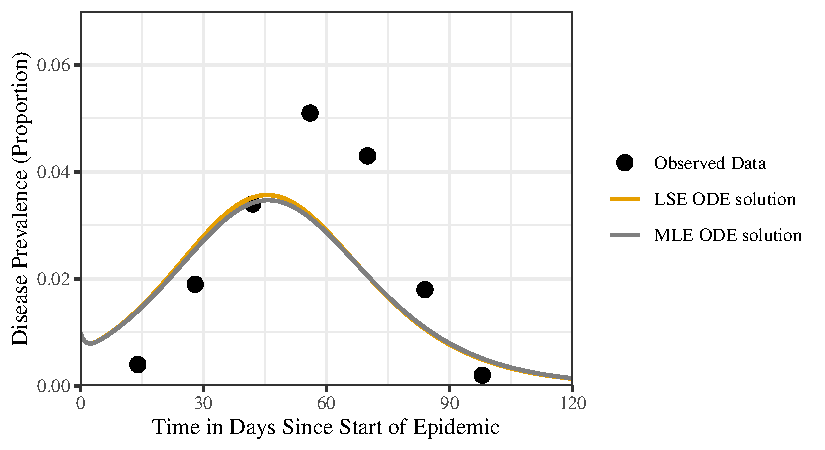
\includegraphics{MLE_SSE_SEIR.pdf}
    \caption{
        An $SEIR$ model fit to some observed prevalence data taken every two
        weeks over a 14 week period, genetated as $I_t/N$ from the $SEIR$
        simulation in Figure \ref{fig:doob_outputs}.
        All parameters were considered known except for $\beta$.
        The least squares estimate (LSE) $\beta^\LS = 0.3516$
        for $\beta$
        was found by solving the model ODEs and numerically minimising the
        square differences between observed prevalences and the ODE prevalences
        (as proportions). Similarly the maximum likelihood estimate
        $\hat{\beta} = 0.3493$ for $\beta$
        was found by assuming the prevalence (times 1000) was binomially
        distributed from 1000 samples with the probability of success being
        equal to $\frac{I_t}{N}.$
    }
    \label{fig:MLE_SSE}
\end{figure}

We demonstrate estimation of one unknown parameter $\beta$ from an $SEIR$ model,
using prevalence data in Figure
\ref{fig:MLE_SSE}. Both $\beta^\LS$ and $\hat{\beta}$ are very close, but do
not fit the data well suggesting fitting the ODEs to a stochastic model
simulation may be a poor choice. This is because at the beginning of an
epidemic the behaviour is very stochastic. Therefore trying to fit an ODE model
to it's stochastic analogue is not necessarily a good idea. The ODEs are more
likely to well approximate the stochastic model when the number of people in
each compartment is high.

\section{Bayesian Parameter Estimation}

In frequentist statistical inference, $\btheta$ is considered to be
fixed, with the observed data $\by^\obs$ assumed to be
generated from a distribution depending on $\btheta.$ Although it is possible
to quantify the uncertainty in parameter estimates through confidence intervals,
frequentist estimates naturally lend themselves to point estimates.
In contrast, inference under a Bayesian
framework assumes that $\btheta$ is also a random variable according to some
pre-known prior distribution. `Evidence' from the observed data then updates
belief about
$\btheta,$ resulting in a posterior distribution of $\btheta,$ described by
Bayes' theorem, namely
$$
    \Pr(\btheta|\by^\obs) \propto \Pr(\by^\obs|\btheta)\Pr(\btheta).
$$

Bayesian parameter estimation is still dependent on the likelihood function
$\mathcal{L}(\btheta) := \Pr(\by^\obs|\btheta).$
With samples from the posterior distribution, we are
able to run our models to capture uncertainty in predicting future scenarios.
For instance, a government may be interested in the number of additional
hospital beds that need to be available to cope with an outbreak of a disease.
If a disease model can be used to approximate outbreaks of the disease,
we can use previous instances of the disease to calibrate our model parameters.
Samples from the posterior parameter distribution, allow
the model to be run multiple times with the varying sets of parameters,
and provide a range of predicted outcomes for the disease. This allows for
confidence in how much investment may be required in the health system.
Similarly, samples from the posterior parameter distribution allow for scenario
modelling such as introducing a new vaccine.

\subsection*{Rejection Sampling}

If we have known ways to sample from the posterior parameter distribution,
then we can use these. However if we have an equation for the probability
distribution, but no way of sampling directly we can sample using rejection
sampling. To sample $X$ through rejection sampling,
we need an explicit way of calculating
$g(x)$ (where $g$ is proportional to the density of $X$), a constant $M$ and
a distribution $p$ such that $Mp(x) \geq g(x)$ with a sampling method
available.

\begin{algorithm}[htbp]
    \caption{Rejection Sampler}
    \label{alg:rej_samp}
    \begin{algorithmic}[1]
        \State Sample $X^\ast \sim p$
        \State Sample $U \sim \mathrm{Unif}(0, 1)$
        \If{$U \leq \frac{g(X^\ast)}{M p(X^\ast)}$}
        \State \Return $X^\ast$ as a sample from the distribution of $X$
        \Else
        \State Repeat
        \EndIf
    \end{algorithmic}
\end{algorithm}

Under this methodology, the distribution function of $X$ is

\begin{align*}
    \Pr(X = x)
    \propto & \Pr(X^\ast = x , U \leq \frac{g(X^\ast)}{M p(X^\ast)})
    \tag*{where the probabilities may be interpreted as densities}                   \\
    =       & \Pr(U \leq \frac{g(X^\ast)}{M p(X^\ast)} | X^\ast = x) \Pr(X^\ast = x) \\
    =       & \frac{g(x)}{M p(x)} p(x)
    =       & \frac{g(x)}{M}
\end{align*}

as required.

\begin{figure}
    \centering
    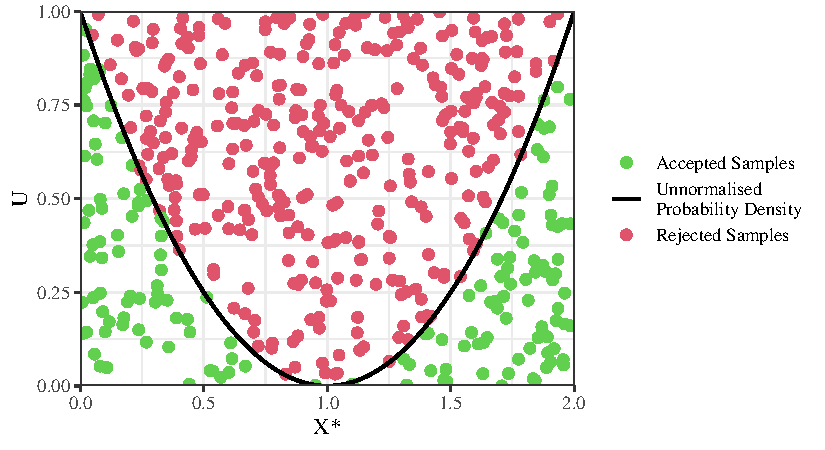
\includegraphics{accept_reject.pdf}
    \caption{
        Samples of $X$ from the unnormalised density $g(x) = (x - 1)^2$ with
        $x\in(0,2)$ using the rejection sampler. $X^\ast\sim\mathrm{Unif}(0,2)$
        and $M = 1.$
        Green dots are samples from
        from $X.$
        Of 500 samples of $X^\ast$, 157 were accepted as samples of $X$.
    }
    \label{fig:accept_reject}
\end{figure}

\begin{example}
    Let $g(x) = (x - 1)^2$ be an unnormalised density function for
    $x \in (0,2).$ $g(x) \leq 1,$ the density of a $\mathrm{Unif}(0,2)$ random
    variable. Therefore to generate samples from $g$ we sample uniformly from
    $X^\ast \sim \mathrm{Unif}(0, 2),$ and then accept the sample if a new
    $U \sim \mathrm{Unif}(0, 1)$ is less than $(X^\ast - 2)^2.$ This is
    demonstrated in \ref{fig:accept_reject}
\end{example}

\subsection*{Markov Chain Monte Carlo Methods}

Often it is not possible to sample directly from the posterior distribution
$\Pr(\btheta|\by^\obs)$ using a rejection sampler, as there is no
explicit form proportional to the true density.
Therefore a common way of sampling from a distribution $p(x)$ is
to construct a Markov chain with stationary distribution $p(x).$
Hence, eventually each new state the
chain moves to will be a be a (not necessarily independent) sample from $p(x),$
or in our case $\Pr(\btheta|\by^\obs).$

\begin{definition}[(Discrete-Time) Markov Chain]
    A sequence of random variables
    $X_0, X_1, \dots$
    is a (discrete-time) \emph{Markov chain} $\{X_i\}_{i\in\mathbb{N}}$ if for
    all
    $k\in\mathbb{N}$,
    $$
        \Pr(X_{i+1}\in A|X_0, X_1, \dots, X_i)
        = \Pr(X_{i+1}\in A|X_i)
    $$
\end{definition}

If $X_i\in\mathcal{X},$ then $\mathcal{X}$ is the state space of the Markov
chain. For example the Markov chain constructed in Figure \ref{fig:MC}, has
discrete state space $\mathcal{X} = \{1, 2\}.$

\begin{figure}[htbp]
    \centering
    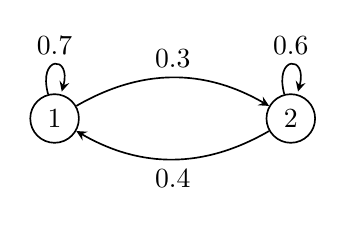
\begin{tikzpicture}[>=stealth, auto, semithick]

        % States
        \node[draw, circle] (A) at (0,0) {1};
        \node[draw, circle] (B) at (3,0) {2};

        % Transitions
        \draw[->] (A) to[bend left] node[above] {0.3} (B);
        \draw[->] (B) to[bend left] node[below] {0.4} (A);
        \draw[->] (A) edge[loop above] node {0.7} (A);
        \draw[->] (B) edge[loop above] node {0.6} (B);

    \end{tikzpicture}
    \caption{
        A simple time homogeneous Markov chain, with two states.
        It is characterised by the transition kernel
        $K(1, 1) = \Pr(X_{i + 1} = 1 | X_i = 1) = 0.7,$
        $K(1, 2) = \Pr(X_{i + 1} = 2 | X_i = 1) = 0.3,$
        $K(2, 1) = \Pr(X_{i + 1} = 1 | X_i = 2) = 0.4,$ and
        $K(2, 2) = \Pr(X_{i + 1} = 2 | X_i = 2) = 0.6.$ The stationary
        distribution is $\pi(1) = 4/7$ and $\pi(2) = 3/7.$
    }
    \label{fig:MC}
\end{figure}

Markov chains are characterised by a transition kernel $K$ with
$$K(x_i, x_{i + 1}) := \Pr(X_{i + 1} = x_{i + 1} | X_i = x_{i + 1}),$$
where this probability is interpreted as a density for continuous random
variables. $K(1, 1)$ would therefore be the probability of going from state 1
to state 2.

We will restrict our focus to Markov chains where
if the value of $X_i$ is known to be $x$, behaviour of chain from this point on
will be identical to the behaviour of the chain from $X_j,$ if this is also
observed to be $x$.

\begin{definition}[Time Homogeneous]
    A Markov chain is \emph{time homogeneous} if
    $$
        \{X_i, X_{i+1}, \dots, X_{i + n}\}
        \overset{d}{=} \{X_{i^\prime}, X_{i^\prime+1}, \dots, X_{i^\prime + n}\}
    $$
    for all $i, i^\prime, n \in \mathbb{N},$ given $X_i = x = X_{i^\prime}.$
\end{definition}

The Markov chain in Figure \ref{fig:MC} is time homogeneous. It doesn't
matter how long it took to get into a state, the Markov chain will behave the
same from that point forward.

\begin{definition}[Stationary Distribution]
    A Markov chain has \emph{stationary distribution} $\pi$ if for $X_i \sim \pi,$
    then $X_{i + 1} | X_i \sim \pi.$
\end{definition}

\begin{example}
    Given the Markov chain in Figure \ref{fig:MC}, the stationary distribution
    can be calculated by solving the simultaneous equations
    \begin{align*}
        K(1, 1) \times \pi(1)
        + K(2, 1) \times \pi(2) = 0.7 \times \pi(1)
        + 0.4 \times \pi(2) = & \, \pi(1) \\
        \pi(1) + \pi(2) =     & \, 1.
    \end{align*}
    Therefore $\pi(1) = 4/7$ and $\pi(2) = 3/7.$
\end{example}

As stated earlier, to sample from a distribution $p(x),$ we construct a Markov
chain with this stationary distribution. A sufficient condition to know that
we have achieved this is if our chain satisfies the the detailed balance
condition.

\begin{theorem}[Detailed balance condition]
    A Markov chain has stationary distribution $p(x),$ which it converges to
    independent of initialisation, if for all $x, x^\prime,$
    $$p(x)K(x, x^\prime) = p(x^\prime)K(x^\prime, x).$$
\end{theorem}

\begin{proof}
    More formally this requires the notions of recurrent, nonnull,
    irreducible and aperiodic which we do not discuss here. For a full
    discussion and proof
    see \cite[chapter 6]{robert_monte_2010}.
\end{proof}

\subsubsection*{Metropolis-Hastings}

The Metropolis-Hastings algorithm is one way of constructing a Markov
chain with stationary distribution equal to the target distribution $g.$
We choose a proposal distribution $q(x^\prime| x)$ which given our last sample
$x,$ generates a new random
variable $X^\prime.$ For example $q$ might be the density of
$X^\prime \sim N(x, 1),$ a normal random variable with mean
around the previous sample. Then similar to rejection sampling, then $X^\prime$
is accepted as the next state in the distribution with some probability
$\alpha$, chosen in such a way that if
$X_i \sim g,$ then $X_{i + 1}\sim g.$ Formally this is set out in
Algorithm \ref{alg:MH}.

\begin{algorithm}[htbp]
    \caption{Metropolis-Hastings Sampler}
    \label{alg:MH}
    \begin{algorithmic}[1]
        \State Initialise $x_0$
        \For{$i = 1$ to $N$}
        \State Sample $X^\prime \sim q(x^\prime|x_{i - 1})$
        \State Compute acceptance ratio
        $\alpha
            = \min\left(
            \frac{
            g(x^\prime) q(x_{i - 1}|x^\prime)
            }{
            g(x_{i - 1}) q(x^\prime|x_{i - 1})
            },
            1
            \right)$
        \State Sample $U \sim \text{Uniform}(0, 1)$
        \If{$U \leq \alpha$}
        \State $x_i \gets X^\prime$
        \Else
        \State $x_i \gets x_{i-1}$
        \EndIf
        \EndFor
        \State \Return $\{x_0, x_1, \dots, x_N\}$
    \end{algorithmic}
\end{algorithm}

Note that for symmetric proposal distributions $q(x^\prime|x) = q(x|x^\prime),$
$\alpha$ simplifies to $\min\left(\frac{g(x^\prime)}{g(x)}, 1\right),$ in
which case the algorithm is simply called a Metropolis sampler.

\begin{theorem}
    The chain produced by Algorithm \ref{alg:MH} $\{X_k\}_{k\in \mathbb{N}}$
    has stationary distribution $g$ for proposal distributions that cover the
    support of $g.$
\end{theorem}

\begin{proof}
    We show that the detailed balance condition
    $$
        g(x)q(x^\prime | x)\alpha(x, x^\prime)
        =g(x^\prime)q(x | x^\prime)\alpha(x^\prime, x)
    $$
    where $\alpha(x, x^\prime) = \min\left(
        \frac{
                g(x^\prime) q(x|x^\prime)
            }{
                g(x) q(x^\prime|x)
            },
        1
        \right)$
    is satisfied. Without loss of generality let
    $g(x^\prime) q(x|x^\prime) < g(x) q(x^\prime|x),$ so
    $\alpha(x, x^\prime) = \frac{
            g(x^\prime) q(x|x^\prime)
        }{
            g(x) q(x^\prime|x)
        },$ and $\alpha(x^\prime, x) = 1.$
    \begin{align*}
        g(x)q(x^\prime | x)\alpha(x, x^\prime)
        = & g(x)q(x^\prime | x) \times \frac{
            g(x^\prime) q(x|x^\prime)
        }{
            g(x) q(x^\prime|x)
        }                                                \\
        = & g(x^\prime) q(x|x^\prime)                    \\
        = & g(x^\prime) q(x|x^\prime)\alpha(x^\prime, x)
    \end{align*}
\end{proof}

\begin{figure}[htbp]
    \centering
    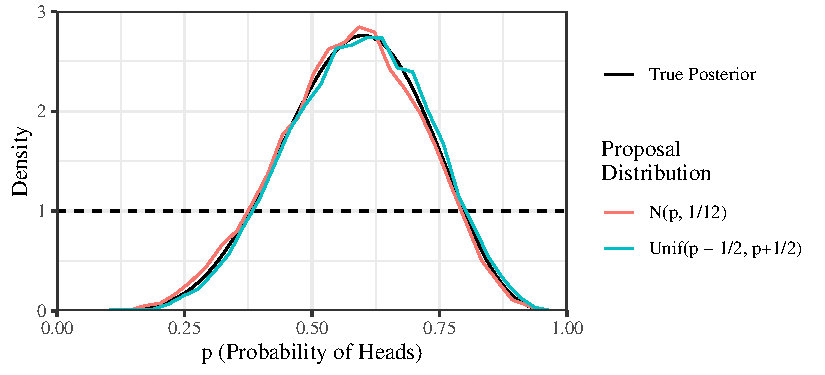
\includegraphics{coin_MH_R.pdf}
    \caption{
        Samples from the posterior distribution of $p$ using the
        Metropolis-Hastings algorithm. $p$ was assumed to
        have a uniform prior between 0 and 1, with $y^\obs = 6,$ generated
        from $\mathrm{Binom}(10, p),$
        The choice of proposal distribution did not impact the final estimate
        of $\Pr(p | y^\obs).$
    }
    \label{fig:coin_R}
\end{figure}

Interestingly, the proof does not depend choice of proposal distribution,
This can be seen in Example \ref{ex:coin_toss} and Figure \ref{fig:coin_R}.

\begin{example}[Coin toss]\label{ex:coin_toss}
    Let the probability of tossing a heads on a weighted coin be
    $\Pr(X = 1) = p.$ Assume that $p\sim \mathrm{Unif}(0,1).$
    We observe $y^\obs = 6$ heads from 10 tosses of the coin.
    Therefore
    $$
        \Pr(p | y^\obs) \propto \Pr(y^\obs| p)\Pr(p)
        = \binom{n}{y^\obs}p^{y^\obs}(1 - p)^{n - y^\obs}\times 1
        = 210p^6(1-p)^4.
    $$
    We sample from this distribution using the Metropolis algorithm which
    becomes
    \begin{algorithmic}[1]
        \State Initialise $p_0$
        \For{$i = 1$ to $N$}
        \State Sample $P^\prime \sim q(p^\prime|p_{i - 1})$
        \State Compute acceptance ratio
        $\alpha
            = \min\left(
            \frac{(P^\prime)^6(1-P^\prime)^4}{p_{i - 1}^6(1-p_{i - 1})^4}, 1
            \right)$ \Comment{Assuming $q$ symmetric}
        \State Sample $U \sim \text{Uniform}(0, 1)$
        \If{$U \leq \alpha$}
        \State $p_i \gets X^\prime$
        \Else
        \State $p_i \gets x_{i - 1}$
        \EndIf
        \EndFor
        \State \Return $\{p_0, p_1, \dots, p_N\}$
    \end{algorithmic}

    We can compare two
    different proposal distributions for $q(p^\prime | p)$,
    $P^\prime \sim N(p, 1/12),$ and
    the second being $P^\prime \sim \mathrm{Unif}(p - 1/2, p + 1/2).$ The first
    1000 samples were discarded as burn in, and it was thinned to every 5
    samples.
    The resulting distribution of the samples can be seen in Figure
    \ref{fig:coin_R}, with both proposal distributions resulting in samples
    that are good at estimating the true distribution.
\end{example}

Since the chain converges to the stationary distribution over time, and is
highly correlated,
a derived chain $\{x_{B + iT}\}_{i \in \mathbb{N}}$ is constructed
from the output. The
first $B$ samples are discarded as `burn in' samples to reduce the impact
of the initialisation point. The chain is `thinned' by taking every $T$th sample,
Since $X_i$ and $X_{i + 1}$ may also be highly correlated (in samples where
the proposed $X^\prime$ is rejected, $X_i = X_{i + 1}$).
This derived chain is considered a
random sample from the target distribution $g.$
In practice, diagnostics such as trace plots and autocorrelation plots are used
to determine $B$ and $T$ are used (see
\cite[chapter 11]{gelman_bayesian_2014}).

\begin{figure}[htbp]
    \centering
    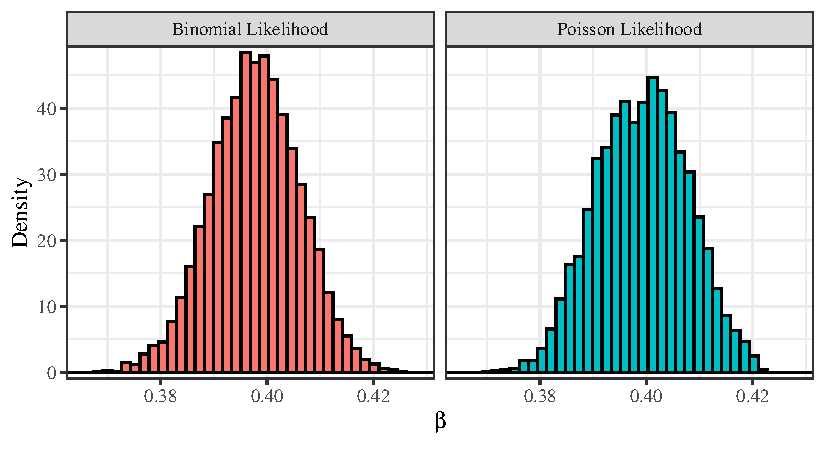
\includegraphics[width=\textwidth]{SIS_beta_pred.pdf}
    \caption{
        Given a daily incidence of $y^\obs = 26$ at day 30 of an $SIS$ epidemic,
        with unknown $\beta,$ we use Metropolis-Hasting to
        sample from $\Pr(\beta | y^\obs).$
        $\gamma = 1/4$ was assumed to be correct, and we compared the assumption
        $y^\obs
            \sim \mathrm{Binom}(\lfloor S_{30} \rfloor,\, \beta I_{30}/N),$
        to the assumption $y^\obs \sim \Pois(\frac{\beta I_{30} S_{30}}{N})$
        where $I_{30}, S_{30}$ are the ODE solutions to Equations
        \ref{eq:SIS_1} and \ref{eq:SIS_2}. We assumed the prior distibution
        $\beta\sim \mathrm{Gamma}(2, 6),$ where $\E(\beta) = 1/3.$ Our proposal
        density was $N(\beta^\ast, 1/10),$ where $\beta^\ast$ was the previous
        sample.
    }
    \label{fig:SIS_MH_R}
\end{figure}

For disease models, given a prior distribution for the parameter(s) $\btheta,$
Metropolis-Hastings can be used to produce samples from
$\Pr(\btheta | y^\obs) \propto \mathcal{L}(\btheta)\Pr(\btheta),$ where
$\mathcal{L}(\btheta)\Pr(\btheta)$ can be calculated to a proportionality
constant but not directly
sampled from. For example given an $SIS$ model with unknown
$\beta \sim \mathrm{Gamma}(2, 6)$ and daily case counts $y^\obs,$ we can
estimate sample from $\btheta | y^\obs$ as in Figure \ref{fig:SIS_MH_R}.

\subsubsection*{Gibbs Sampling}

\begin{algorithm}[htbp]
    \caption{Gibbs Sampler}
    \label{alg:gibbs}
    \begin{algorithmic}[1]
        \State Initialise
        $\btheta^{(0)} = (\theta_1^{(0)}, \theta_2^{(0)}, \dots, \theta_d^{(0)})$
        \For{$i = 1$ to $N$}
        \State Sample
        $\theta_1^{(i)}
            \sim \Pr(
            \theta_1
            | \theta_2^{(i-1)}, \theta_3^{(i-1)}, \dots, \theta_d^{(i-1)}
            )$
        \State Sample
        $\theta_2^{(i)}
            \sim \Pr(
            \theta_2
            | \theta_1^{(i)}, \theta_3^{(i-1)}, \dots, \theta_d^{(i-1)})$
        \State $\vdots$
        \State Sample
        $\theta_d^{(i)}
            \sim \Pr(
            \theta_d
            | \theta_1^{(i)}, \theta_2^{(i)}, \dots, \theta_{d-1}^{(i)})$
        \State Save $(\theta_1^{(i)}, \theta_2^{(i)}, \dots, \theta_d^{(i)})$
        as $\btheta^{(i)}$
        \EndFor
        \State \Return $\{\btheta^{(0)}, \btheta^{(1)}, \dots, \btheta^{(N)}\}$
    \end{algorithmic}
\end{algorithm}

Some models, may have a parameters such that it is possible
to sample from $\theta_1 | \theta_2, \by^\obs$, and
$\theta_2 | \theta_1, \by^\obs$ but not the joint distribution of
$(\theta_1, \theta_2)| \by^\obs.$ A (multidimensional) Markov chain can be
constructed by iteratively updating the parameters. Such a method is called
a Gibbs sampler, described in
Algorithm \ref{alg:gibbs}. The distribution of the Markov chain
sampler will eventually converge to the
$\Pr(\theta_1, \theta_2 | \by^\obs),$ and for the same reasons as for
the Metropolis-Hastings
sampler, after thinning and discarding burn in, we consider the resulting
chain a sequence of independent samples from our target distribution.

\begin{theorem}[Gibbs Sampler]
    The Markov chain generated by Algorithm \ref{alg:gibbs}
    converges to the distribution of $\Pr(\btheta|\by^\obs).$
\end{theorem}

\begin{proof}
    We prove that the Gibbs Sampler satifies the detail balance
    equation for two unknown parameters.
    The transition kernel of the Markov chain is
    $$
        q(\btheta^{(i)}|\btheta^{(i-1)})
        := \Pr(\theta^{(i)}_1 | \theta^{(i-1)}_2, \by)
        \Pr(\theta^{(i)}_2 | \theta^{(i)}_1, \by).
    $$

    To prove the detailed balance condition is satisfied, we need to show that
    $$
        \Pr(\btheta^{(i-1)}| \by)q(\btheta^{(i)}|\btheta^{(i-1)})
        = \Pr(\btheta^{(i)}| \by)q(\btheta^{(i - 1)}|\btheta^{(i)}).
    $$

    \begin{align*}
        \Pr(\btheta^{(t-1)}| \by)q(\btheta^{(i)}|\btheta^{(i-1)})
        = & \, \Pr(\theta_1^{(i-1)}, \theta_2^{(i-1)}| \by) \times
        \Pr(\theta^{(i)}_1 | \theta^{(i-1)}_2, \by) \times
        \Pr(\theta^{(i)}_2 | \theta^{(i)}_1, \by)                        \\
        = & \, \Pr(\theta_1^{(i-1)}| \theta_2^{(i-1)}, \by) \times
        \Pr(\theta_2^{(i-1)}| \by) \times
        \Pr(\theta^{(i)}_1 | \theta^{(i-1)}_2, \by) \times
        \Pr(\theta^{(i)}_2 | \theta^{(i)}_1, \by)                        \\
        = & \, \Pr(\theta_1^{(i-1)}| \theta_2^{(i-1)}, \by) \times
        \Pr(\theta^{(i)}_1, \theta^{(i-1)}_2 | \by) \times
        \Pr(\theta^{(i)}_2 | \theta^{(i)}_1, \by)                        \\
        = & \, \Pr(\theta^{(i)}_2 | \theta^{(i)}_1, \by) \times
        \Pr(\theta^{(i)}_1, \theta^{(i-1)}_2 | \by) \times
        \Pr(\theta_1^{(i-1)}| \theta_2^{(i-1)}, \by)                     \\
        = & \, \Pr(\theta^{(i)}_2 | \theta^{(i)}_1, \by) \times
        \Pr(\theta^{(i)}_1 | \by)  \times
        \Pr(\theta^{(i-1)}_2 | \theta^{(i)}_1, \by) \times
        \Pr(\theta_1^{(i-1)}| \theta_2^{(i-1)}, \by)                     \\
        = & \, \Pr(\theta^{(i)}_1, \theta^{(i)}_2| \by) \times
        \Pr(\theta^{(i-1)}_2 | \theta^{(i)}_1, \by) \times
        \Pr(\theta_1^{(i-1)}| \theta_2^{(i-1)}, \by)                     \\
        = & \, \Pr(\btheta^{(t)}| \by) q(\btheta^{(i -1)}|\btheta^{(i)})
    \end{align*}
    as required, so the posterior pdf $\Pr(\btheta|\by)$ is the unique
    stationary pdf associated with the generated Markov chain.
\end{proof}

\begin{figure}[htbp]
    \centering
    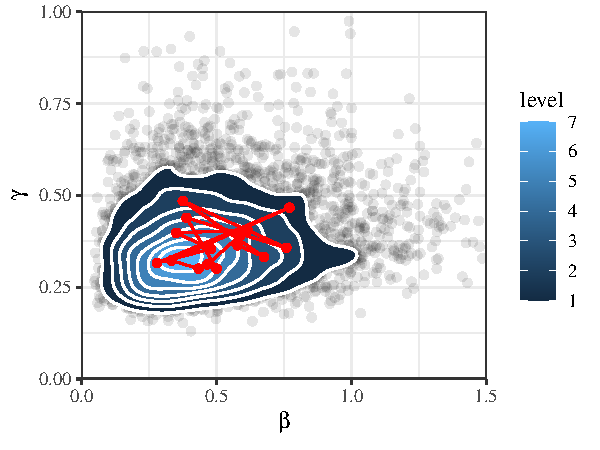
\includegraphics{SIS_gibbs.pdf}
    \caption{
        2000 posterior samples from $\Pr(\beta, \gamma | \by^\obs),$ where
        $\beta|\gamma, \by^\obs
            \sim \mathrm{Gamma}(9, 4/\gamma + 4 + 8\gamma)$ and
        $\gamma|\beta, \by^\obs
            \sim \mathrm{InvGamma}(12, 12\beta).$ The samples were
        obtained using a Gibbs sampler.
        The red points are the first 15 samples using the Gibbs sampler.
    }
    \label{fig:gibbs_R}
\end{figure}

\begin{example}
    Consider the $SIS$ model described by equations \ref{eq:SIS_1}
    and \ref{eq:SIS_2}. Early in an epidemic, the average number of new
    cases generated from a single infectious individual is known as $R_0.$
    This can be shown to be $\frac{\beta}{\gamma}$ for the $SIS$ model.
    Let $\by^\obs = \{1, 1, 3, 1\}$ be the number of people infected by four
    different individuals at the start of the epidemic. We assume that the
    number of infections are generated from a Poisson distribution with mean
    $\frac{\beta}{\gamma}.$ Therefore the likelihood
    $$
        \mathcal{L}(\beta, \gamma):= \Pr(\by^\obs | \beta, \gamma)
        = \frac{
            \left(\frac{\beta}{\gamma}\right)^{1 + 1 + 3 + 1}
            \exp( -\frac{4\beta}{\gamma})
        }{
            1!\times 1! \times 3! \times 1!
        }
        \propto\left(\frac{\beta}{\gamma}\right)^{6}\exp( -\frac{4\beta}{\gamma})
    $$
    Let us assume that from similar previous epidemics we assume that
    $\beta | \gamma \sim \mathrm{Gamma}(3, 4 + 8\gamma),$ and
    $\gamma | \beta \sim \mathrm{InvGamma}(6, 8\beta).$ Therefore
    \begin{align*}
        \Pr(\beta|\gamma, \by^\obs)
        \propto & \Pr(\by^\obs|\gamma, \beta)\Pr(\beta|\gamma)      \\
        \propto &
        \left(\frac{\beta}{\gamma}\right)^{6}
        \exp( -\frac{4\beta}{\gamma})
        \times \beta^{3 - 1}\exp(-(4 + 8\gamma)\beta)               \\
        \propto & \beta^{9 - 1}\exp(-(4/\gamma + 4 + 8\gamma)\beta)
    \end{align*}
    and so
    $\beta|\gamma, \by^\obs
        \sim \mathrm{Gamma}(9, 4/\gamma + 4 + 8\gamma).$
    Similarly
    \begin{align*}
        \Pr(\gamma|\beta, \by^\obs)
        \propto & \Pr(\by^\obs|\gamma, \beta)\Pr(\gamma|\beta)         \\
        \propto &
        \left(\frac{\beta}{\gamma}\right)^{6}
        \exp( -\frac{4\beta}{\gamma})
        \times \gamma^{- 6 - 1}\exp\left(-\frac{8\beta}{\gamma}\right) \\
        \propto & \gamma^{- 12 - 1}
        \exp\left(-\frac{12\beta}{\gamma}\right)
    \end{align*}
    and so
    $\gamma|\beta, \by^\obs
        \sim \mathrm{InvGamma}(12, 12\beta).$
    Now we have explicit forms for the conditional probabilities,
    we generate samples using the Gibbs sampler in Algorithm \ref{alg:gibbs}.
    Samples from the distribution can be seen in Figure \ref{fig:gibbs_R}
\end{example}

The Gibbs sampler and Metropolis-Hastings sampler are often combined, by
using a Metropolis-Hastings sampler for each step of the conditional sampling.
This is useful when the conditional distributions
$\Pr(\theta_1 | \theta_2, \by^\obs)$ can be calculated up to a proportionality
constant, but not directly sampled from.

\subsection*{Approximate Bayesian Computation}

So far, under a Bayesian framework, parameter estimation has still been
dependent on the likelihood function
$\mathcal{L}(\btheta) := \Pr(\by^\obs|\btheta)$ through Bayes' theorem.
In many cases, such as stochastic disease models and agent based models, the
likelihood has no explicit form, or is intractable to calculate. 
In this case we can still
sample $\by(\btheta),$ with likelihood $\Pr(\by^\obs | \btheta)$ by definition.

Therefore